\section{度量空间的比较}
\label{sec:mmap-comparison}

两个度量空间“一样”是什么意思，取决于我们要保留什么。若要保留每一对点的距离，就要求映射保持距离；若只要保留开集、收敛与紧性，同胚就够了；若要保留柯西列与完备性，或者进一步保留误差的数量级，就需要介于两者之间的条件。

本节先研究保持距离的映射，再说明同胚为什么不保留完备性，最后在同一集合的两个度量之间，把“等价”分成三个强弱不同的层次。

\subsection{等距映射}
\label{sec:mmap-isometry}

最强的比较是要求距离完全不变。

\begin{definition}[等距映射]
\label{def:mmap-isometry}
若映射$f:X\to Y$对所有$x,x'\in X$满足
\begin{equation}
 d_Y(f(x),f(x'))=d_X(x,x'),
 \label{eq:mmap-isometry}
\end{equation}
则称$f$为\term{等距映射}（isometric mapping），也称\term{等距嵌入}（isometric embedding）。若等距映射还是满射，称$X$与$Y$等距。
\end{definition}

等距映射自动是单射：$f(x)=f(x')$时，由式~\eqref{eq:mmap-isometry}得$d(x,x')=0$。它是$1$-Lipschitz的，因而连续。由于距离不变，$(x_n)$是柯西列当且仅当$(f(x_n))$是柯西列，$x_n\to x$当且仅当$f(x_n)\to f(x)$。

把$f$看成$X$到像集$f(X)$的双射，它的逆也是等距映射。于是$X$完备当且仅当子空间$f(X)$完备，$X$紧致当且仅当$f(X)$紧致：这些性质都只用距离和点列描述，经等距映射原样搬运。

满射与否区分了“相同”与“嵌入”。平面的旋转和平移都是$(\mathbb R^2,d_2)$到自身的满射等距映射，旋转前后的图形作为度量空间无法区分。$t\mapsto(t,0)$是$\mathbb R$到$\mathbb R^2$的等距映射，但不是满射，它把实轴嵌成平面中的一条直线。第~\ref{chap:metric-spaces}章完备化中的$\iota:X\to\hat X$也是等距嵌入，它的像稠密，只有$X$本身完备时才是满射。

无限空间可以等距地嵌入自身的真子集，有限集做不到这一点。在自然数集$\{1,2,\ldots\}$上取通常距离，$n\mapsto n+1$保持距离，但像集不含$1$。所以“$X$等距嵌入$Y$且$Y$等距嵌入$X$”不能直接推出两者等距，需要单独核验满射。

\subsection{同胚与度量性质}
\label{sec:mmap-homeomorphism-metric}

第~\ref{chap:topological-spaces}章的同胚是双向连续的双射，它保持一切用开集表述的性质，例如紧致、连通、可分，以及点列的收敛。那里还说明了实轴与开区间同胚，这里取从实轴到开区间的方向：
\begin{equation}
 h:\mathbb R\to(-1,1),\qquad
 h(x)=\frac x{1+\lvert x\rvert},\qquad
 h^{-1}(y)=\frac y{1-\lvert y\rvert}.
 \label{eq:mmap-homeo-h}
\end{equation}

图~\ref{fig:mmap-homeo-line}画出$h$对整数点的作用。两个空间都配上通常的距离$\lvert\cdot\rvert$。上方整数点相邻间距恒为$1$，下方的像却越来越挤，集中到端点$1$。

\begin{BookInlineFigure}
  \centering
  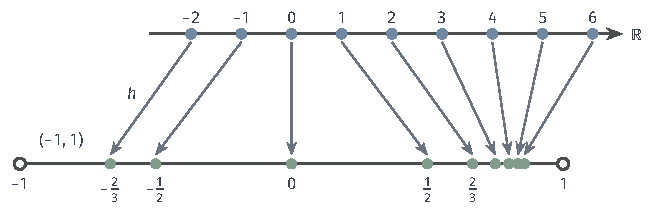
\includegraphics[width=110.659mm]{figures/04-spaces-measures-and-geometry/01-topology-and-metric/tikz/mmap-homeo-line/figure.pdf}
  \caption{同胚$h(x)=x/(1+\lvert x\rvert)$把$\mathbb R$上的整数点（上方，蓝）映到开区间$(-1,1)$内（下方，绿）。上方点列相邻距离恒为$1$，不是柯西列；像点$1-1/n$是柯西列，但极限$1$不在开区间内。}
  \label{fig:mmap-homeo-line}
\end{BookInlineFigure}

$\mathbb R$完备，$(-1,1)$不完备：$y_n=1-1/n$是$(-1,1)$中的柯西列，极限$1$不在其中。用$h^{-1}$搬回实轴，
\[
 h^{-1}(y_n)=\frac{1-1/n}{1/n}=n-1,
\]
相邻两项相距$1$，不是柯西列。同胚把一个柯西列变成了非柯西列，所以柯西性不是拓扑性质，完备性也不是。同样，$(-1,1)$有界、全有界，$\mathbb R$两者都不是，所以有界性与全有界性也不被同胚保持。

换一个角度，同一个集合也可以配上拓扑相同、完备性不同的度量。在$\mathbb R$上令
\[
 d_h(x,y)=\lvert h(x)-h(y)\rvert.
\]
$h$是单射，所以$d_h$是度量；$h:(\mathbb R,d_h)\to(-1,1)$是满射等距映射，所以$(\mathbb R,d_h)$不完备，其中$x_n=n-1$是柯西列而无极限。

另一方面，$h$是通常拓扑下的同胚，$d_h$的开集恰是通常的开集。这就是第~\ref{chap:metric-spaces}章预告的、与通常度量拓扑相同却不完备的度量。

在紧致度量空间之间，这种差别不会出现：紧致蕴含完备且全有界，而紧致是拓扑性质，所以与紧致度量空间同胚的度量空间也完备、全有界。差别只出现在非紧空间中，那里完备性依赖于“无穷远处”的距离怎样度量。

\subsection{同一集合上的度量等价}
\label{sec:mmap-metric-equivalence}

设$d$与$d'$是同一集合$X$上的两个度量。比较它们相当于研究恒等映射$\operatorname{id}:(X,d)\to(X,d')$及其逆满足什么条件。按要求由弱到强，有三种“等价”。

\begin{definition}[度量的三种等价]
\label{def:mmap-metric-equivalence}
设$d,d'$是$X$上的度量。
\begin{enumerate}
\item 若$d$与$d'$诱导相同的开集，即$\operatorname{id}$双向连续，称它们\term{拓扑等价}（topologically equivalent）；
\item 若$\operatorname{id}:(X,d)\to(X,d')$与其逆都均匀连续，称它们\term{一致等价}（uniformly equivalent）；
\item 若存在常数$0<c\leq C$，使对所有$x,y$有
\begin{equation}
 c\,d(x,y)\leq d'(x,y)\leq C\,d(x,y),
 \label{eq:mmap-strong-equivalence}
\end{equation}
即$\operatorname{id}$双向Lipschitz连续，称它们\term{强等价}（strongly equivalent）。
\end{enumerate}
\end{definition}

由Lipschitz连续蕴含均匀连续、均匀连续蕴含连续，强等价蕴含一致等价，一致等价蕴含拓扑等价。三个层次分别保留不同的信息，表~\ref{tab:mmap-metric-equivalence}是一份汇总，下面逐一解释。

\begin{BookInlineTable}
  \centering
  \caption{同一集合上三种度量等价保留的信息}
  \label{tab:mmap-metric-equivalence}
  \begin{tabular}{lll}
    \toprule
    等价层次 & 保留的性质 & 不保留的性质 \\
    \midrule
    拓扑等价 & 收敛点列、紧致、可分 & 柯西列、完备 \\
    一致等价 & 另加柯西列、完备、全有界 & 有界性 \\
    强等价 & 另加有界集、误差尺度 & 常数$c,C$的具体值 \\
    \bottomrule
  \end{tabular}
\end{BookInlineTable}

拓扑等价保留一切拓扑性质。按序列判据，它等价于两个度量下收敛的点列及其极限完全相同，所以紧致、可分以及映射的连续性都不因换用另一个度量而改变。它不保留柯西列：上一小节的$\lvert\cdot\rvert$与$d_h$拓扑等价，但前者完备、后者不完备。

一致等价还保留柯西列与完备性。均匀连续映射把柯西列送到柯西列，恒等映射双向均匀连续，两个度量下的柯西列就相同，而收敛点列本来就相同，所以一个完备当且仅当另一个完备。

它还保留全有界性。给定$\varepsilon$，由$\operatorname{id}:(X,d)\to(X,d')$的均匀连续性取$\delta$，则
\[
 B_d(x,\delta)\subseteq B_{d'}(x,\varepsilon),
\]
$d$下半径$\delta$的有限覆盖就是$d'$下半径$\varepsilon$的覆盖；反方向同理。

一致等价却不保留有界性。$\mathbb R$上的$\lvert x-y\rvert$与$\min\{\lvert x-y\rvert,1\}$在小于$1$的尺度上完全一致，对$\varepsilon<1$取$\delta=\varepsilon$，就得到双向均匀连续。但后者下整个$\mathbb R$有界，而前者下$\mathbb R$无界，所以不存在$c>0$使$\min\{\lvert x-y\rvert,1\}\geq c\lvert x-y\rvert$对所有$x,y$成立。

强等价进一步比较误差的尺度。由式~\eqref{eq:mmap-strong-equivalence}，
\begin{equation}
 B_d(x,r/C)\subseteq B_{d'}(x,r)\subseteq B_d(x,r/c),
 \label{eq:mmap-ball-sandwich}
\end{equation}
所以两个度量下的有界集相同，覆盖数也只差一个尺度因子：
\[
 N^{d'}(C\varepsilon,A)\leq N^{d}(\varepsilon,A),
\]
其中上标表示所用的度量。

$\mathbb R^n$上的$\rho_\infty$与$d_2$是最常见的例子，它们满足
\[
 \rho_\infty(\bm x,\bm y)\leq d_2(\bm x,\bm y)\leq\sqrt n\,\rho_\infty(\bm x,\bm y).
\]

取$n=2$，$d=d_2$，$d'=\rho_\infty$，则$c=1/\sqrt2$，$C=1$。把$r=1$代入式~\eqref{eq:mmap-ball-sandwich}，得
\[
 B_{d_2}(\bm x,1)\subseteq B_{\rho_\infty}(\bm x,1)\subseteq B_{d_2}(\bm x,\sqrt2).
\]
图~\ref{fig:mmap-balls}画出的就是这三个集合：圆盘、外切正方形，以及外接圆盘。

\begin{BookInlineFigure}
  \centering
  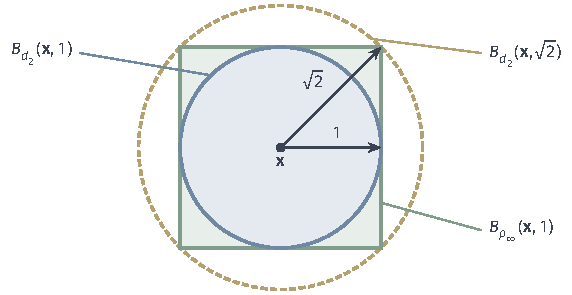
\includegraphics[width=96.852mm]{figures/04-spaces-measures-and-geometry/01-topology-and-metric/tikz/mmap-balls/figure.pdf}
  \caption{$\mathbb R^2$上强等价的两个度量。蓝色圆盘是$d_2$的单位球，绿色正方形是$\rho_\infty$的单位球，黄色虚线圆是$d_2$的半径$\sqrt2$的球。正方形夹在两个圆盘之间，比例由常数$c=1/\sqrt2$，$C=1$决定。}
  \label{fig:mmap-balls}
\end{BookInlineFigure}

卷二证明了有限维空间上任意两个范数诱导的度量都强等价，所以在有限维空间中说“收敛”“有界”“完备”无需指明范数；估计误差时则要记得常数$c,C$可能依赖于维数。这一点在无限维时不再成立，第~\ref{chap:function-normed-spaces}章将看到同一函数空间上不等价的范数。

文献中“等价度量”有时指拓扑等价，有时指强等价。本书遇到这一说法时会写明是哪一种，或直接写出所要求的映射条件。
